\section{Mémoire}
\commentaire{Idées en cours ainsi que re formulation}


De nombreux systèmes IoT déjà présents sur les voitures trouvent également leur place sur les motos, tels que l’alerte d’angle mort, l’ABS, l’anti-patinage ou encore le contrôle de traction. Toutefois, malgré ces points communs, des différences significatives subsistent entre ces deux types de véhicules, notamment dans leur comportement et leurs contraintes spécifiques. Dans cette partie, je vais concentrer mon analyse sur l’évaluation de la route et sur les moyens d’optimiser la prise de trajectoire.


% faire des schémas avec les trajectoires pour souvelver les problèmes

\subsection{Pratique de la route - Analyse comparative des besoins de sécurité entre voitures et motos}

\commentaire{\\
Analyse des différences fondamentales : protection physique, stabilité, visibilité, comportements routiers.\\
	•	Quelles fonctionnalités IoT des voitures sont difficilement transférables ?\\
•	Quelles fonctionnalités sont transférables mais nécessitent adaptation ?\\
•	Mise en évidence des lacunes spécifiques aux motos.
}

J’ai eu l’occasion d’expérimenter la pratique du deux-roues sous différents angles :\
\begin{itemize}
    \item Les trajets du quotidien,
    \item Les balades entre ami(e)s,
    \item Les road trip de plus d'une dizaine de jours (environ 200 à 300 kms par jour), souvent en milieu montagneux.
\end{itemize}
Avec plus de 35 000 km parcourus en deux ans, voici les constats que j’ai pu faire autour de moi :
\begin{itemize}
  \item Les trajets du quotidien peuvent paraître anodins, mais c’est justement la routine qui les rend dangereux. En connaissant la route par cœur, on a tendance à relâcher sa vigilance, alors que les risques restent bien réels (état de la chaussée, comportement imprévisible des autres usagers, etc.).
  \item Les balades entre ami(e)s apportent un vrai plaisir de conduite, mais l’effet de groupe peut parfois inciter à dépasser ses limites. On peut se retrouver à rouler à des vitesses inadaptées ou à prendre de mauvaises décisions sous l’influence de comportements plus audacieux. Le jugement individuel peut alors être altéré.
  \item Les road trips, quant à eux, demandent une grande endurance. La fatigue s’accumule rapidement, et avec elle, le temps de réaction s’allonge. Il est essentiel d’être pleinement en possession de ses capacités pour pouvoir réagir correctement en cas de situation imprévue.
\end{itemize}
Enfin, un point important : lorsque la chaussée est mouillée, la majorité des motards adoptent naturellement une conduite plus prudente, vitesse réduite, prise d’angle limitée, meilleure anticipation. Cela montre que la perception du risque influence fortement le comportement. %transition
Abordons maintenant une difficulté que beaucoup de deux-roues rencontres: les virages.

\subsubsection{Étude des virages}
%TRAJECTOIRES SECURITÉ
\commentaire{idée : montrer que c'est complexe}
Les illustrations ci-dessous représentent différentes trajectoires dites de sécurité. Ce sujet occupe une place centrale dans les campagnes de prévention menées par les acteurs de la sécurité routière. Il est régulièrement abordé par les forces de l’ordre, notamment les gendarmes spécialisés dans la sécurité des deux-roues motorisés, mais également par les formateurs, les auto-écoles et les usagers eux-mêmes.\\
En effet, la trajectoire de sécurité constitue une technique de conduite essentielle pour limiter les risques en virage, optimiser la visibilité et mieux anticiper les éventuels dangers. Elle permet au motard d’adopter une position plus stratégique sur la chaussée, en tenant compte à la fois du tracé de la route, de l’environnement, et de la circulation en sens inverse.\\
La sensibilisation à cette pratique est donc fortement encouragée, que ce soit lors des formations initiales, des stages post-permis ou à travers les communications des institutions publiques. Les illustrations présentées ici ont pour but de mieux comprendre ces trajectoires et de visualiser les choix possibles selon différents contextes routiers.
\begin{figure}[H]
    \centering
    \includegraphics[width=0.4\textwidth]{coeur_memoire/schéma/trajectoire_sécurité_1.png} 
    \caption{Trajectoire de sécurité utilisée sans obstacle}
\end{figure}
Adopter une trajectoire comme celle illustrée ci-dessus permet principalement d’optimiser la visibilité à l’entrée et dans le cœur du virage. En s’éloignant légèrement de l’intérieur de la courbe, le motard bénéficie d’un champ de vision plus large, ce qui lui permet d’anticiper plus facilement les éventuels obstacles, les changements d’adhérence ou la présence d’un autre usager.
Toutefois, cette trajectoire doit être adaptée dès lors qu’un autre véhicule circule en sens inverse. Dans ce cas, la priorité n’est plus uniquement la visibilité, mais également la sécurité du croisement. Il convient alors d’adopter une trajectoire dite de compromis ou "de sécurité", qui permet de conserver une marge de manœuvre tout en maintenant une distance suffisante avec le véhicule opposé.\\
La figure suivante illustre ainsi la trajectoire idéale à privilégier en présence d’un autre usager sur la route. Elle vise à garantir un passage fluide, sans empiétement sur la voie opposée, tout en maintenant une bonne stabilité du deux-roues dans la courbe. Ce type d’ajustement est essentiel pour réduire les risques de collision frontale, notamment dans les virages à visibilité réduite.
\begin{figure}[H]
    \centering
    \includegraphics[width=0.4\textwidth]{coeur_memoire/schéma/trajectoire_sécurité_4.png} 
    \caption{Trajectoire de sécurité utilisée avec un autre usager}
\end{figure}
Instinctivement, le motard va se rapprocher à l'extérieur du virage pour s'éloigner du danger représenté en bleu par la voiture.
Pour poursuivre cette démonstration, nous allons y ajouter d'autres dangers sur la route représentés par des objets en bleu rendant l'impossibilité de prendre une trajectoire "parfaite". Dans la vie courante, cela peut représenter des gravillons, un animal mort sur la route, des plaques d'égout, des nids de poule, des bandes d'étanchéité (mastics), etc. Ces éléments font perdre de suite l'adhérence des pneus et peuvent entraîner une chute. 
\begin{figure}[H]
    \centering
    \includegraphics[width=0.4\textwidth]{coeur_memoire/schéma/trajectoire_sécurité_2.png} 
    \caption{Autre configuration de la route avec plusieurs autres dangers}
\end{figure}
Ajoutons maintenant la trajectoire idéale à la situation permettant de garder l'adhérence des pneus:
\begin{figure}[H]
    \centering
    \includegraphics[width=0.4\textwidth]{coeur_memoire/schéma/trajectoire_sécurité_3.png} 
    \caption{Trajectoire de sécurité utilisée avec des dangers sur la route}
    \label{fig:trajectoire_securite_difficulte}
\end{figure}
Cette trajectoire améliore l’adhérence des pneus, mais elle présente un risque important en cas de danger venant en sens inverse. Si un véhicule surgit en face, le motard dispose de très peu de temps pour réagir ou se décaler, ce qui peut entraîner un accident. Il est donc essentiel d’adapter sa trajectoire en fonction de plusieurs éléments : l’état de la route, la visibilité et la présence d’autres usagers. La vitesse joue également un rôle déterminant : plus la moto roule vite, plus il devient difficile de corriger la trajectoire à temps. Voici ci-dessous plusieurs exemples de trajectoires, chacune présentant ses avantages et ses limites.
\begin{figure}[H]
  \centering
  \begin{subcaptionbox}{Trajectoire possible 1}[0.4\linewidth]
    {\includegraphics[width=\linewidth]{coeur_memoire/schéma/trajectoire_sécurité_7.png}}
  \end{subcaptionbox}
  \hfill
  \begin{subcaptionbox}{Trajectoire possible 2}[0.4\linewidth]
    {\includegraphics[width=\linewidth]{coeur_memoire/schéma/trajectoire_sécurité_6.png}}
  \end{subcaptionbox}
  
  \vspace{0.5cm}
  
  \begin{subcaptionbox}{Trajectoire possible 3}[0.4\linewidth]
    {\includegraphics[width=\linewidth]{coeur_memoire/schéma/trajectoire_sécurité_5.png}}

  \end{subcaptionbox}

  \caption{Autres exemples de trajectoires de sécurité}
\end{figure}

Annalysons et commentons ces trajectoires:\
\begin{itemize}
    \item Trajectoire 1 : C’est la plus sécurisante. Elle permet de s’éloigner efficacement du véhicule venant en sens inverse. Toutefois, si la vitesse est trop élevée, il sera difficile de revenir à l’intérieur du virage, comme le montre la trajectoire en vert.
    \item Trajectoire 2 : Elle est plus risquée, car elle place le motard plus près du danger potentiel. Même si la courbe semble fluide et permet une prise de virage à vitesse plus élevée, elle réduit la marge de manœuvre en cas d’imprévu.
    \item Trajectoire 3 : Elle représente un bon compromis, car elle maintient une certaine distance avec les véhicules en face. Cependant, rester trop proche du bas-côté peut s’avérer dangereux, notamment en cas d’obstacle imprévu (dégradation de la chaussée, présence d’un animal, etc.). La visibilité y est également plus restreinte, ce qui peut compromettre l’anticipation, l'analyse du virage.
\end{itemize}
Pour conclure sur ces schémas, il existe de nombreuses trajectoires possibles, mais peu sont réellement adaptées aux spécificités de la conduite moto. Certaines sont plus risquées que d’autres, et l’expérience du pilote joue un rôle clé dans le choix et la gestion de la trajectoire. Cela met en évidence à quel point cette phase de conduite est exigeante et complexe et combien de facteurs doivent être pris en compte pour envisager une assistance efficace.

%ETUDE SONDAGE
\subsubsection{Enquête auprès de motards - Recueil de ressenti}
J'ai réalisé une enquête dans différents groupes de motards sur les réseaux sociaux afin de récupérer leur ressenti. Il est très important pour comprendre la problématique de s'intéressé à l'intéressé. Cela m'a permis de mieux comprendre leurs besoins, leurs attendus afin d'avoir un oeil beaucoup plus objectif de ce que moi je peux vivre, ressentir. L'échantillon est composé d'une petite vingtaine de personnes avec 58,8 \% d'hommes contre 41,2 \% de femmes.
Voici les différents profils des participants :
\begin{figure}[H]
  \centering
  \begin{subcaptionbox}{Age des participants}[0.5\linewidth]
    {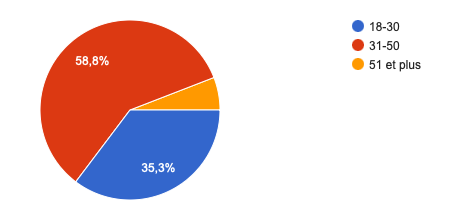
\includegraphics[width=\linewidth]{coeur_memoire/graphique/age.png}}
  \end{subcaptionbox}
  \hfill
  \begin{subcaptionbox}{Nombre d'années de permis}[0.5\linewidth]
    {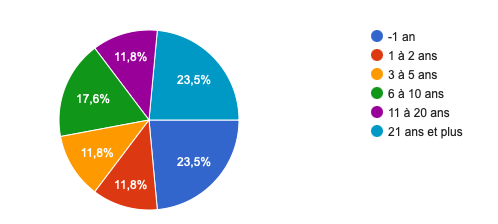
\includegraphics[width=\linewidth]{coeur_memoire/graphique/nb_annees_permis.png}}
  \end{subcaptionbox}

  \begin{subcaptionbox}{Nombre de kms à l'année}[0.5\linewidth]
    {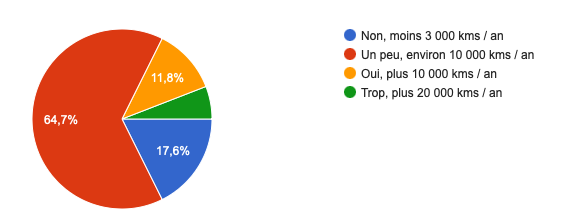
\includegraphics[width=\linewidth]{coeur_memoire/graphique/nb_km_an.png}}
  \end{subcaptionbox}
  \hfill
  \begin{subcaptionbox}{Utilisation de la moto}[0.5\linewidth]
    {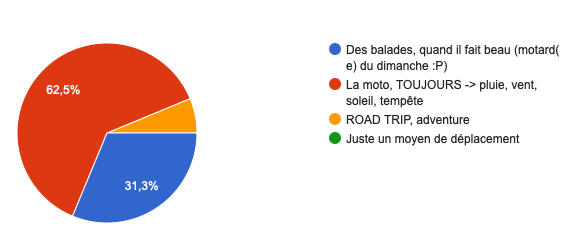
\includegraphics[width=\linewidth]{coeur_memoire/graphique/utilisation_moto.png}}
  \end{subcaptionbox}
  \caption{Profils des participants}
\end{figure}

Pour conclure, lors de cette enquête, il y a tous types de motards. Beaucoup roulent moins de 3 000 kms/an ce qui est très peu. C'est moins d'expérience sur la route.
Lors de mon enquête, la plupart des usagers possèdent des deux-roues roadster comme des 400 cc à 600 cc. On retrouve des Honda, Kawasaki, Aprillia, KTM et Yamaha. Ce sont des motos qui sont inférieures à 10 000 euros.
Pour les voyages, ou bien les voyages dans les Alpes, j'ai pu apercevoir une majorité de motards qui roulent en GS\footnote{Gelände/Straße : tout-terrain/route. C'est une moto conçue pour être à la fois confortable sur route et capable de rouler sur des chemins non goudronnés. Premiers prix : 12 000 euros, haut de gamme : environ 30 000 euros.}. J'estime entre environ 50 et 70\% des motos rencontrées dans les Alpes (Suisse, Italie et France) sont des GS.\\
Voici quelques retours d'expérience des motards en situation d'urgence selon l'enquête :\\
• "Proche d'un rond-point, j'ai mal évalué la distance. Donc je suis arrivée trop vite, j'étais déjà dans l'insertion sur le rond-point et j'ai failli terminer dans un véhicule. Contrainte d'effectuer un freinage d'urgence et de me mettre le plus à l'extérieur pour éviter la catastrophe."\\
• "La voiture de La Poste stationnée en plein virage en sens inverse, empiétant sur ma voie. Sur une route à 50 km/h en agglomération. J'ai dû pratiquer l'évitement pour ne pas me prendre le véhicule."\\
• "Ma roue s’est coincée dans un rail de tram .. "\\
• "J'ai pris un trou (pas visible avant d'être dedans) sur une nationale, ce qui m'a fait guidonner, impossible à rattraper donc la moto a fini par se coucher et une belle glissade pour finir."\\
• "Évitement de personne qui tourne sans avoir mis de clignotant. Classique."
\vspace{0.5cm}

Pour la fin de l'étude, j'ai demandé aux participants quelles sont leurs attentes concernant les technologies IoT sur les motos. Certains ne souhaitent pas de technologie IoT, car ils estiment que cela peut nuire à la conduite et à la sensation de liberté. D'autres sont favorables à l'intégration de technologies IoT. Par exemple, un assistant virtuel qui indiquerait au pilote les dangers potentiels sur la route (chausée dégradée, virage dangereux, gravillon...). Les autres retours sont des technologies qui sont déjà présentes sur les motos du marché comme l'ABS, le contrôle de traction, l'anti-patinage, etc. Cependant, d'après certains motards, il faut mettre ces éléments de série et non en option comme l'appel d'urgence.
\vspace{0.5cm}

De plus, les réseaux sociaux relaient régulièrement des actualités concernant des accidents impliquant des deux-roues, illustrant la vulnérabilité des motards. Par exemple, un article (Voir ~\ref{articlemoto}) récent publié par Ouest-France rapporte qu'une jeune femme de 26 ans a perdu tragiquement la vie lors d'une leçon de moto-école dans l’Ain. L'accident s'est produit le samedi 2 août 2025 près de Châtillon-la-Palud. Alors qu'elle circulait sur une portion de route comportant plusieurs virages, elle a perdu le contrôle de son véhicule et percuté violemment une glissière de sécurité. La jeune femme n’a pas survécu à ses blessures. Aucun autre véhicule ne serait impliqué. Ce tragique événement rappelle une fois de plus l’importance d'améliorer constamment la sécurité des motards et l'importance de savoir bien aborder un virage.
\vspace{0.5cm}

Le véritable défi réside dans la capacité à adapter la trajectoire en temps réel, en fonction d’un ensemble de paramètres dynamiques et interdépendants. Cette adaptation ne dépend pas uniquement de la courbure de la route, mais également de nombreux vecteurs qui rendent la situation complexe à modéliser et à anticiper. Parmi ces vecteurs, on peut citer :\\
\begin{itemize}
\item La vitesse instantanée du véhicule, qui influence directement la trajectoire possible et le temps de réaction du conducteur ;
\item L’angle d’inclinaison de la moto, déterminant l’équilibre et l’adhérence lors de la prise de virage ;
\item L’état de la chaussée, incluant l’adhérence, les irrégularités, les débris ou l’humidité ;
\item Les conditions météorologiques, telles que la pluie, le vent, la chaleur ou le brouillard, qui impactent à la fois la visibilité et la tenue de route ;
\item La présence et le comportement des autres usagers, qu’il s’agisse de véhicules motorisés, de cyclistes ou de piétons ;
\item La géométrie de la route, incluant la largeur, le dénivelé, les virages successifs ou les intersections.
\end{itemize}
Dans ce contexte complexe, les technologies IoT (Internet of Things) peuvent jouer un rôle central. En fournissant des données en temps réel sur l’environnement routier, elles permettent de mieux analyser la situation et de faciliter la prise de décision. Par exemple, une communication entre véhicules pourrait alerter un motard d’un freinage brusque à venir, ou un capteur pourrait ajuster une recommandation de trajectoire en fonction de l’adhérence mesurée sur la route.\\
Il est important de rappeler que, malgré les apports technologiques, la trajectoire la plus appropriée reste celle dans laquelle le motard se sent en sécurité. Elle dépend fortement de son expérience, de ses réflexes, de sa confiance en lui et de sa connaissance de la route. Il n’existe donc pas une seule "bonne" trajectoire, mais une pluralité d’options, à ajuster en fonction du contexte, des données disponibles et des capacités du pilote.

%PLAISIR
\subsubsection{Défi passion}
\vspace{0.5cm}
Le plaisir de conduire une moto réside dans la sensation de liberté qu'elle procure. Cependant, cette liberté s'accompagne de responsabilités, notamment en matière de sécurité. Les technologies IoT peuvent contribuer à améliorer cette sécurité tout en préservant le plaisir de conduite. "Passionné auto moto depuis mon plus jeune âge, j'aime rouler souvent seul, mais j'aime me sentir libre et pouvoir aller où je veux et quand je veux, la moto, c'est indescriptible et c'est comme une drogue, mais c'est la passion." selon un retour de l'enquête.

\vspace{0.5cm}
Adapter l'IOT représente un défi car il faut prendre en compte de nombreux paramètres (environnement, comportement des usagers, etc.) et s'assurer que les solutions proposées sont adaptées à chaque situation.

\newpage
\subsection{ Étude critique des technologies IoT existantes (voitures vs motos)}
\commentaire{\\
avec un regard critique et des cas concrets.\\
Analyse de cas réels où les technologies IoT ont été adaptées à la moto (Airbags connectés, gilets intelligents, casques IoT, etc.).\\
  Freins techniques : taille réduite, alimentation électrique, exposition météo, vibrations, etc.\\
  lidar et radar ?\\
}

\subsubsection{Exemples d’IoT adaptés et développé pour la moto}
Plusieurs dispositifs connectés ont été développés spécifiquement pour les motards ces dernières années. Voici quelques exemples :
\begin{itemize}
  \item Airbags connectés (ex. : Dainese Smart Jacket, In\&motion avec Ixon): Ces gilets intelligents détectent les mouvements anormaux (chute, décélération brutale) via accéléromètres et gyroscopes, et déclenchent un coussin gonflable. L’algorithme est souvent connecté à une plateforme cloud qui analyse les données de milliers d’utilisateurs pour améliorer la détection.
  \item Casques connectés (ex. : CrossHelmet, Shoei IT-HT, Livall): Ils embarquent caméras arrière, GPS, commandes vocales, HUD\footnote{affichage tête haute} et parfois même des alertes de proximité de véhicules. Certaines marques permettent la communication entre motards via Bluetooth ou 4G.
  \item Systèmes d’aide à la navigation : Solutions telles que Calimoto, TomTom Ride... Offrent une navigation simplifiée pensée pour les deux-roues, avec une interface minimaliste et résistante aux intempéries.
\end{itemize}
Ces exemples illustrent que l’écosystème IoT appliqué à la moto progresse mais demeure nettement moins mature que celui dédié à l’automobile. Il serait donc pertinent de mesurer concrètement l’impact de ces technologies sur la sécurité, en s’appuyant sur des données chiffrées. Par exemple, quantifier la baisse du nombre de blessures graves grâce à l’utilisation d’airbags intelligents permettrait de dépasser le simple discours technologique pour appuyer les bénéfices réels.
La question de l’accessibilité reste également centrale. Le coût élevé de certains équipements comme un casque connecté pouvant varier entre 500 et 1500 euros peut représenter un frein pour de nombreux motards. De plus, la complexité liée à l’installation, à la configuration ou à la mise à jour de ces dispositifs peut décourager leur adoption à grande échelle.

\subsubsection{Les radars}
Aujourd'hui, de nombreuses motos sont équipées de technologies directement issues de l’industrie automobile, telles que l’ABS (système antiblocage des roues), la détection d’angle mort ou encore le régulateur de vitesse adaptatif. Ces dispositifs ont été progressivement adaptés pour répondre aux contraintes spécifiques des deux-roues, en tenant compte des enjeux liés à l'équilibre, à la maniabilité et à la sécurité du motard.
Après avoir expérimenté ces technologies, les retours des utilisateurs sont globalement très positifs. Ils mettent notamment en avant le gain en confort, particulièrement sur les longs trajets ou dans les conditions difficiles. Le régulateur adaptatif, par exemple, réduit significativement la fatigue en ajustant automatiquement la vitesse en fonction du véhicule qui précède. La détection d’angle mort accroît quant à elle la vigilance du conducteur, permettant une meilleure anticipation des dangers et réduisant ainsi les risques de collision.\\
L'intégration de ces technologies améliore non seulement l’expérience de conduite, mais contribue également de manière concrète à la sécurité routière. Moins sollicités sur des tâches répétitives, les motards conservent une meilleure concentration et sont donc moins exposés aux erreurs liées à la fatigue ou à l’inattention. Ces progrès montrent clairement l'intérêt de continuer à développer et à adapter des technologies automobiles avancées aux besoins spécifiques des utilisateurs de deux-roues motorisés.\\
%LIDAR
Les radars sont aujourd’hui intégrés aux modèles les plus récents de motos et remplissent efficacement leur fonction. Comme mentionné précédemment, la détection des éléments présents sur la route joue un rôle essentiel dans la sécurité du motard, tout comme les actions automatisées ou assistées qui en découlent. Ces technologies permettent notamment d’anticiper certains dangers, d’éviter des collisions ou de réguler la vitesse en fonction de l’environnement immédiat.\\
Cependant, les radars présentent certaines limites. Leur capacité à différencier les types d’objets ou à analyser finement l’environnement reste restreinte. C’est dans ce contexte que l’utilisation du LiDAR (Light Detection and Ranging) s’avère particulièrement intéressante. Cette technologie repose sur l’émission de faisceaux laser pour mesurer avec grande précision les distances et modéliser l’environnement en trois dimensions. Elle est très performante pour la cartographie 3D et la classification des objets, ce qui en fait un atout majeur dans les systèmes d’aide à la conduite avancés.\\

Néanmoins, le LiDAR n’est pas sans contraintes. Il reste très sensible aux conditions météorologiques défavorables telles que la pluie, le brouillard ou la neige, qui peuvent altérer la qualité des données recueillies. De plus, son intégration sur une moto pose plusieurs défis pratiques. La taille et le poids des capteurs peuvent affecter la maniabilité, l’esthétique et l’ergonomie de la moto. Sans compter le coût : en 2020, selon PW Consulting\cite{marche_capteur_lidar}, un capteur LiDAR compact se situait entre 3 000 et 10 000 euros — un prix difficilement envisageable pour la majorité des motards.\\

Heureusement, les coûts tendent à diminuer avec l’évolution du marché et la démocratisation de cette technologie. Aujourd’hui, il est possible de se procurer un capteur LiDAR pour un montant compris entre 500 et 2 000 euros, en fonction des gammes et des performances souhaitées. Cela ouvre de nouvelles perspectives pour une intégration progressive sur les deux-roues, à condition que les autres contraintes techniques soient également maîtrisées.\\

\vspace{0.5cm}
Les prototypes :\\
\begin{table}[ht]
\centering
\begin{tabular}{|l|c|}
  \hline
  Éléments & Prix \\
  \hline
  Capteurs LIDAR & 500 à 2 000 euros \\
  Traitement embarqués & 300 à 1 500 euros \\
  Interfaces et boîtier durci & 100 à 400 euros \\
  Intégration et calibration & 200 à 1 000 euros \\
  Total estimation & 1 100 à 5 900 euros \\
  \hline
\end{tabular}
\caption{Prix moyen estimé pour la technologie LIDAR sur moto (2025)}
\end{table}

Prenons les coûts moyens d'un deux roues :\\
\begin{table}[ht]
\centering
\begin{tabular}{|l|c|c|}
\hline
\textbf{Catégorie} & \textbf{Cylindrée} & \textbf{Prix moyen (TTC, €)} \\
\hline
Scooter & 50--125 cm³ & 2\,000 -- 4\,500 euros \\
Moto légère & 125 cm³ & 3\,500 -- 5\,000 euros \\
Moto moyenne cylindrée & 300--650 cm³ & 6\,000 -- 9\,000 euros \\
Moto grosse cylindrée & 700--1 000+ cm³ & 10\,000 -- 18\,000 euros \\
Moto sportive haut de gamme & 1 000+ cm³ & 18\,000 -- 30\,000 euros \\
Moto électrique & équiv. 50--125 cm³ & 4\,000 -- 12\,000 euros \\
\hline
\multicolumn{2}{|c|}{\textbf{Prix moyen toutes catégories}} & \textbf{7\,000 -- 9\,000 euros} \\
\hline
\end{tabular}
\caption{Prix moyen estimé des deux-roues neufs en 2025 (France/Europe) par The Market Reports}
\end{table}

\subsubsection{GPS}
Aujourd’hui, les systèmes GPS intégrés aux voitures ont atteint un haut niveau de maturité. Ils offrent une expérience fluide, fiable et parfaitement adaptée aux besoins de la conduite automobile. Les GPS modernes embarquent des composants hautement performants : un récepteur GNSS\footnote{Global Navigation Satellite System : capte les signaux émis par les satellites GPS, Galileo, GLONASS ou BeiDou pour calculer la position.}, des antennes optimisées, ainsi que des processeurs et chipsets de navigation capables d’interpréter rapidement les données satellites et d’exécuter des algorithmes de positionnement précis. L’ensemble est complété par des haut-parleurs intégrés, permettant de recevoir des instructions vocales sans quitter la route des yeux.
La situation est bien différente pour les motos. Ici, aucun habitacle ne protège contre la pluie, la poussière, les vibrations ou les chocs. Un GPS moto doit donc être conçu pour résister à ces contraintes. Cela implique l’utilisation d’un boîtier étanche et renforcé, conforme aux normes IP67/IP68\footnote{Les indices IP67 et IP68, définis par la norme IEC 60529, indiquent le niveau de protection d’un appareil contre la pénétration de poussière et d’eau.}, ainsi qu’un système de fixation robuste pour supporter les conditions de roulage. Les vibrations du moteur et de la route peuvent en effet détériorer des composants qui, dans un environnement automobile stable, ne subiraient aucun dommage.

\subsubsection{Contraintes techniques et comparaison voitures vs motos dans l’adoption des technologies IoT}

L’intégration de solutions IoT diffère fortement entre voitures et motos, en raison de contraintes physiques, énergétiques et environnementales propres à chaque type de véhicule. Le tableau \ref{tab:comparaison_iot_voiture_moto} présente une vue d’ensemble, suivie d’une analyse détaillée des points clés pour les deux-roues.

\begin{table}[H]
\centering
\caption{Comparaison des conditions d’intégration des technologies IoT entre voitures et motos}
\label{tab:comparaison_iot_voiture_moto}
\renewcommand{\arraystretch}{1.15}
\begin{tabular}{|p{3.2cm}|p{6.5cm}|p{6.5cm}|}
\hline
\textbf{Critère} & \textbf{Voiture} & \textbf{Moto} \\
\hline
\textbf{Espace disponible} &
Suffisant pour intégrer de nombreux composants électroniques (capteurs, unités de calcul, caméras, etc.) &
Très limité, surtout sur les modèles sportifs ou compacts ; intégration plus contraignante \\
\hline
\textbf{Alimentation électrique} &
Batterie de forte capacité alimentant de multiples systèmes &
Batterie réduite, imposant des dispositifs sobres en énergie \\
\hline
\textbf{Protection matérielle} &
Composants protégés par un habitacle fermé &
Composants exposés aux intempéries, à la poussière, aux vibrations et aux variations thermiques \\
\hline
\textbf{Sécurité passive} &
Ceintures, airbags frontaux et latéraux, zones de déformation &
Gilet airbag externe, casque et protections mécaniques personnelles \\
\hline
\textbf{Ergonomie d’affichage} &
Écrans tactiles, HUD, commandes vocales &
Affichage minimaliste via smartphone, casque connecté ou retour haptique/sonore \\
\hline
\textbf{Maturité des technologies IoT} &
Avancée (ADAS, V2X, LIDAR, conduite autonome partielle) &
Émergente (casques connectés, gilets intelligents, radars adaptatifs) \\
\hline
\end{tabular}
\end{table}

Pour les motos, la compacité des composants est un enjeu majeur : chaque capteur, antenne ou processeur doit être discret pour préserver l’esthétique et la maniabilité. La faible capacité électrique impose l’utilisation de modules économes en énergie. Les équipements doivent également résister à un environnement exigeant : exposition directe à la pluie, aux rayons UV, à la poussière et aux projections, avec un indice de protection d’au moins IP67 pour garantir la fiabilité.
Les vibrations et chocs, dus au moteur et à l’état de la route, nécessitent des fixations robustes et des matériaux résistants à l’usure. L’ergonomie est aussi déterminante : l’affichage des données, qu’il soit intégré au tableau de bord ou au casque, doit rester lisible et non distrayant. Ces contraintes cumulées expliquent que, malgré un fort potentiel en matière de sécurité et de confort, certaines innovations IoT restent encore peu démocratisées sur deux-roues.


\subsubsection{Pistes pour intégrer l’IoT dans les deux-roues}
Pour surmonter les limites actuelles, plusieurs pistes peuvent être envisagées :
Miniaturisation : développer des capteurs IoT plus petits et moins gourmands, spécifiques aux motos.
Énergie autonome : utiliser des solutions rechargeables ou solaires intégrées aux équipements (casque, gilet).
Normes de résistance : généraliser des composants certifiés IP67 ou supérieurs.
Interface modulaire : privilégier des alertes visuelles/sensorielles simples (LED, vibration, son), modulables par l’utilisateur.
Systèmes d’analyse distribués : partager les calculs entre un smartphone, un capteur embarqué et le cloud pour alléger la charge locale.
\vspace{0.5cm}

Pour conclure, la technologie LIDAR peut représenter à elle seule entre 12\% et 84\% du prix d'un deux-roues neuf mais le pourcentage reste moindre pour des voitures haut de gamme avoisinant les 50 000 euros. Cela reste très élevé pour un motard, surtout si l'on considère que la majorité des motards ne changent pas de moto tous les ans. De plus, il faut prendre en compte le coût de l'assurance, de l'entretien, du carburant, etc. Il est donc essentiel de trouver un équilibre entre sécurité et coût pour rendre ces technologies accessibles à tous les motards.

%Autre IOT
Concernant les autres technologies que peuvent proposer les autres marques, elles sont très pertinentes car elles sont destinées pour la sécurité des deux-roues et parfois élaborées par des motards eux-mêmes. Je pense à Géoride par exemple, qui est une application complète.\\
Ce qui peut être intéressant est d'avoir une interopérabilité entre les différents systèmes IoT. Prenons l'exemple de Géoride qui a un système de détection de chute, des motos peuvent l'avoir également ainsi que l'intercom Cardo. Cela permettrait d'éviter trois appels.

\subsection{ Proposition d’adaptation technologique}
\commentaire{	\\
•	Systèmes de communication V2X (Vehicle-to-Everything) pour motos : miniaturisation, portabilité, est ce que cela est possible ? les conditions.\\
	•	Capteurs embarqués sur la moto et sur le pilote (gilet, casque, smartphone).\\
	•	Intégration d’IA pour la détection du risque en temps réel : freinage d’urgence, angle d’inclinaison, anticipation de collision. => a voir\\
	•	Systèmes d’alerte connectés avec autres usagers (voitures, infrastructures).\\
	•	Possibilité d’un écosystème IoT dédié aux motos, interopérable avec celui des voitures. => à voir si ca existe déja\\
  • modélisation d'un tableau de bord connecté pour moto, avec des capteurs et des alertes en temps réel.\\
}

%PROPOSITION 1 : GPS MOTO 
\todo{parler également de l'accélération}

Pour pouvoir proposer de nouvelles fonctionnalités de prévention, il faut optimiser le tableau de bord. Il faut créer des logos communs à tous pour avoir le même langage. 

\todo{ajout d'un tableau de bord connecté avec des capteurs et des alertes en temps réel.}
L'idée serait d'intégrer dans les motos une puce GPS qui serait capable d'avertir en cas de virage dangeureux. L'alerte (sonore via un intercom et voyant au tableau de bord) serait envoyée via le tableau de bord connecté si la vitesse est supérieure à la vitesse recommandée. Cette vitesse sera calculée via la valeur de la courbure du virage. Des chercheurs Alex Liniger et Simon Hecker ont développé un prototype , Aegis Rider AG\cite{vitesse_virage_mcnews} permettant de prendre la meilleure trajectoire. Cependant, ce dernier ne prend pas en compte les autres facteurs de la route (autres usagers, état de la chaussée, etc.). Comme démontré ci-dessous, la trace bleu indiquant la trajectoire de sécurité et le compteur de vitesse masquent la qualité de la route par conséquent, le motard ne pourra pas anticiper les dangers de la route (gravillon, trous, ....). À l'heure d'aujourd'hui, cette solution reste extrêmement complexe. Ma solution permettra de fonctionner dans la pluspart des cas.

\begin{figure}[h]
    \centering
    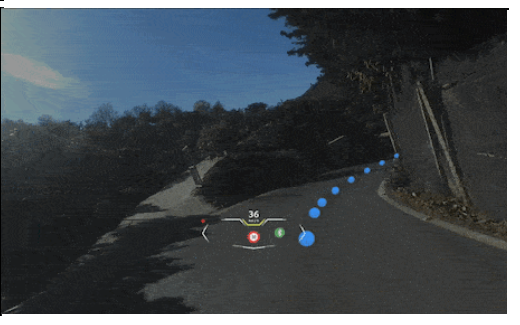
\includegraphics[width=0.7\textwidth]{coeur_memoire/images/aegis.png} 
    \caption{Prototype Aegis Rider AG pour la détection de virages dangereux.}
\end{figure}
Cette fonctionnalité est très interessante mais elle empêche une bonne visibilité de la surface de la route et elle peut fausser une prise de décision.
Comme illustré dans la Figure~\ref{fig:trajectoire_securite_difficulte}, le processus ne pourra pas adapter sur des virages dit "imparfaits".


\todo{voir pour faire une petite ligne de code ?}

\underline{Contexte:} En balade dans le 77, un motard roule sur une départementale. Dans cette situation, il est équipé d'un boitié GPS qui récupère ses coordonnées en temps réel. Il arrive dans une portion de virages limitée à 70 km/h nommée "Les 17 virages", près d'Arbonne-La-Forêt. Cette série de virages est dangeureuse car la route n'est pas bonne, n'est pas large et l'adhérence n'est pas optimale. De plus, il y a un virage dangereux à l'équerre qui surgit au milieu de cette série. La trajectoire de sécurité est fortement recommandé. Par expérience, avoisiner les 70 km/h est déjà bien au vue de la portion qui y est technique.

\begin{figure}[H]
    \centering
    \includegraphics[width=0.7\textwidth]{coeur_memoire/schéma/Capture d’écran 2025-07-24 à 15.45.48.png} 
    \caption{Point GPS des 17 virages.}
\end{figure}

\todo{photo des 17 virages}



Les coordnnées GPS sont : 48.385171, 2.563108.

\todo{mettre le diagramme}
Voici le diagramme d'action de cette fonctionnalité:\\

\begin{figure}[H]
    \centering
    \includegraphics[width=0.8\textwidth]{coeur_memoire/schéma/Capture d’écran 2025-07-24 à 17.48.10.png} 
    \caption{Diagramme d'action du Système de prévention de virages dangereux}
\end{figure}

Pour réaliser un bout de code sur cette fonctionnalité, j'ai décidé d'utiliser ces bibliothèques :\\
• osmnx\cite{osm_doc} : permet d’interroger OSM (OpenStreetMap) et de récupérer des graphes routiers.\\
•	geodesic (de geopy \cite{geopy}) : mesure la distance réelle (en mètres) entre 2 points GPS.\\

L'interêt de calculer la courbure de la courbe est de pouvoir anticiper le virage et par conséquent, adapter la vitesse pour optimiser l'adhérence, la trajectoire où l'on se sentira le plus en sécurité. \\
Le calcul de la courbure permettra d'identifier un virage s'il est dangereux à partir de données GPS cartographiques pour enfin adapter le comportement du système embarqué (alerte, adaptation de trajectoire, assistance..).
Donc la courbure mesure à quel point une route peut changer de direction sur une courte distance, ici, dans un virage.\\
Une route droite a une courbure environ égale à 0. Une route qui tourne fort (virage serré) a une courbure élevée.

\begin{table}[ht]
\centering
\begin{tabular}{|l|c|c|c|}
\hline
Route & Rayon du virage & Courbure (simplifiée) & Risque \\
\hline
ligne droite & infini & 0 & faible \\
Virage large autoroute & 500 m & Faible (0.01) & faible \\
Virage serré en montagne & 30 m & Forte (0.1–0.2) & Élevé \\
\hline
\end{tabular}
\caption{Exemple en pratique}
\end{table}

Un virage serré avec une courbure > 0.1 est souvent dangereux à +60 km/h, surtout à moto.
Plusieurs études indiquent que les rayons < 50 m sont classés comme virages dangereux pour les motos. À plus de 60 km/h, une moto doit pencher à plus de 35°à 40° dans le virage ce qui augmente énormément le risque de chute, surtout s’il y a du gravier, pluie, vent latéral…
L’estimation “courbure > 0.1 = danger > 60 km/h” est une règle empirique, basée sur des données de sécurité moto reonnues, des normes d'ingénierie routière et des approximations géométriques issues de GPS.


L'avantage d'avoir un calcul automatique et en amont, cela permet de prévenir avant même d'être dans le virage. Il peut remplacer un panneau quand celui-ci n'est pas visible. Elle ne remplace pas une analyse dynamique complète mais elle est suffisante pour alerter automatiquement le pilote ce qui est exactement l’objectif du système.



\begin{tcolorbox}[title=Calcul de la courbure]
Courbure mathématique\cite{formule_curvature} d’un virage:
\[
courbure\_virage = \kappa = \frac{1}{R}
\]
où R est le rayon du virage\\
Forme simplifiée de la courbure basée sur la déviation par rapport à une ligne droite.\\
a, b et c sont trois points dans la courbe.\\
\[
curvature = abs((a + b - c) / (a + b))
\]
a + b = distance réelle parcourue en suivant la route \\
c = distance directe entre le début et la fin (comme si on traçait une corde)
\end{tcolorbox}

\begin{figure}[H]
    \centering
    \includegraphics[width=0.7\textwidth]{coeur_memoire/schéma/Capture d’écran 2025-07-22 à 16.27.35.png} 
    \caption{Schéma présentant une moto avant un virage}
\end{figure}


\todo{illustration, développement}

\todo{Détailler le code}

\lstinputlisting[language=Python]{coeur_memoire/programme1.py}


\todo{résultat}
Suite de la mise en situation réelle. Les passages étudiés ont été réalisé bien avant l'expérience, par conséquent, il n'y a aucune notion de vitesse. Chaques passages ont été faits sur la capacité au moment t de l'usager. Voici un premier passage à 51 km/h.
\begin{figure}[H]
    \centering
    \includegraphics[width=0.6\textwidth]{coeur_memoire/images/Capture d’écran 2025-07-28 à 15.56.58.png} 
    \caption{Premier passage dans Les 17 virages}
\end{figure}

Résultat du premier passage avec le programme :
\begin{figure}[H]
    \centering
    \includegraphics[width=0.6\textwidth]{coeur_memoire/images/Capture d’écran 2025-07-28 à 16.23.05.png} 
    \caption{Premier passage dans Les 17 virages}
\end{figure}

Voici maintenant un second passage réalisé un peu plus vite.
\begin{figure}[H]
    \centering
    \includegraphics[width=0.6\textwidth]{coeur_memoire/images/Capture d’écran 2025-07-28 à 16.35.23.png} 
    \caption{Deuxième passage dans Les 17 virages}
\end{figure}


\begin{figure}[H]
    \centering
    \includegraphics[width=0.6\textwidth]{coeur_memoire/images/Capture d’écran 2025-07-24 à 16.20.18.png} 
    \caption{Deuxième passage dans Les 17 virages}
\end{figure}

Le deuxième passage est réalisé plus rapidemment (sans excès de vitesse), cependant, la vitesse est trop "rapide" et nécessite de meilleures capacités pour le passer. Il faut que le motard soit à un niveau bien intermédiaire. Comme l'objectif du programme est de faire de la prévention, j'ai décidé de baser sur un niveau de débutant. Pour conclure, il y a un message qui apparaît.

L'idée maintenant est de prévenir l'usager d'un logo universel. Évidemment, la disposition sera optimisée pour chaque écran. Nous pouvons également y ajouter un bip sonore, cela évitera de fixer en permanance le tableau de bord.
\begin{figure}[H]
    \centering
    \includegraphics[width=0.6\textwidth]{coeur_memoire/images/Capture d’écran 2025-07-25 à 14.42.42.png} 
    \caption{Génération d'un tableau de bord possible avec l'IA.}
\end{figure}



\newpage
\subsection{ Étude de faisabilité et limites}
\commentaire{\\
    •	Quels obstacles (coût, poids, énergie, connectivité, acceptabilité des motards) à l’implémentation ?\\
	•	Quelles pistes pour la recherche ou le développement industriel ?\\
	•	(une maquette fonctionnelle, un prototype conceptuel, ou même une étude de cas simulée)\\
  •	ouverture défi environnemental\\
  •	 protection des données sensibles (lien via kappa)        }


\subsubsection{Objectif de l'étude}
Cette étude vise à évaluer la faisabilité de la mise en œuvre d’un système d’assistance à la conduite basé sur l’analyse de la courbure de la route, dans le but de recommander une vitesse adaptée. Le système exploite des données géographiques pour déterminer la géométrie des segments routiers en fonction de la position d’un véhicule. Puis, il applique un modèle simple de calcul de courbure pour estimer la dangerosité d’un virage et proposer une vitesse conseillée. Ce chapitre examine les obstacles techniques, les contraintes d’implémentation réelle, ainsi que les perspectives de développement.

\subsubsection{Faisabilité technique}
Mon programme utilise des données routières open source via OpenStreetMap (OSM). Ces données sont accessibles et gratuites cependant, on apperçoit un manque de précision surtout en milieu rural. Certains segments peuvent manquer de points ou contenir des simplifications qui faussent l’évaluation de la courbure.
La méthode mise en œuvre repose sur le calcul géodésique entre trois points consécutifs, p1, p2 et p3 sur un segment de route à partir d'un point GPS, la position actuelle. Cela permet d’obtenir une estimation simple de la courbure.
Cependant, cette approche reste sensible à la densité des points sur les segments (peu de points donc cela implique une mauvaise précision).

\subsubsection{Faisabilité d’implémentation sur un véhicule réel}
Le monde du deux-roues posent certaines contraintes matérielles et logicielles :\\
\begin{tabular}{|l|l|}
\hline
\textbf{Élément} & \textbf{Détail} \\
\hline
Capteurs & Nécessité d’un GPS de bonne précision, module RTK pour éviter les erreurs de localisation.\\
Matériel embarqué & Un microcontrôleur\footnote{ (ex : Raspberry Pi, Arduino, ESP32) capable d’exécuter les traitements de calcul ou de les transmettre à une plateforme distante.}\\
Consommation & Ne doit pas être trop importante car ça reste un "petit véhicule" \\
Connectivité & Si les cartes ne sont pas embarquées, une connexion réseau est nécessaire, ce qui pose des limites en zone blanche.\\
\hline
\end{tabular}


Les limites actuellement restent les prix. En effet, ajouter des fonctionnalités de sécurité ayant des prix trop important baissent l'attractivité des motos. 

Comme il n’existe pas encore de produit commercial alliant GPS et l'alerte virage, on peut estimer sur la base des coûts de prototypes et de composants.\\

\begin{tabular}{|l|l|}
\hline
\textbf{Élément} & \textbf{Estimation de coût} \\
\hline
Capteur GPS + IMU (accéléro/magnétomètre)  & 50–200 € \\
Abonnement cartes HD (HERE, TomTom, etc.) &    10–30€ par mois   \\
Interface casque ou écran moto (HUD/haptique) au besoin & 100–300€ \\
\hline
\end{tabular}

\vspace{0.5cm}
Afin d'avoir un GPS précis et réactif. Il doit être accompané de la technologie IMU. IMU permet de compenser la latence et les imprécisions GPS en fournissant la vitesse angulaire (gyroscope) pour la courbure des virages, l'orientation (magnétomètre) et l'accélération linéaire (accéléromètre) pour les freinage. L'IMU peut fonctionner à 100-1000 Hz ce qui permet d'améliorer fortement le temps de réaction. Ces points sont crutiaux pour une fonctionnalité comme la notre, la prédiction d'abord de virages dangereux. La marge d'erreur n'est pas permise.

\vspace{0.5cm}
Voici un tableau comparatif:\\
\begin{tabular}{|c|c|c|}
\hline
\textbf{Propriétés} & \textbf{GPS} & \textbf{GPS + IMU} \\
\hline
Précision position & Environ 3 à 5 m & Bonne \\
Temps de réaction & Lent (de 0,5 à 1 seconde) & Rapide (<0,1 seconde)\\
Fiabilité en virage & Faible & Haute \\
Sensibilité du signal & Oui & Moins critique \\
\hline
\end{tabular}

\vspace{0.5cm}
L’acceptabilité d’un tel système dépend également du profil du conducteur. Un motard préfèrera un système non intrusif (affichage sur smartphone, retour haptique) et intuitif. Le système doit être discret afin de ne pas distraire l’attention ni le surcharger d’information. Un bip, un logo pourraient constituer une solution ergonomique.



\subsubsection{Prototype et simulation}

\subsubsection{Limites et contraintes}




\todo{mon programme}
Le programme fonctionne dans la pluspart des cas. Cependant, les données liant la limitation de vitesse n'est pas toujours récupérée. Par conséquent, par défaut la limitation de vitesse est 80 km/h. Sur les portions d'autoroute, la limitation est de 130 km/h et la courbure a une valeur quasiment nulle. Prenons un cas où la limitation est 110 km/h, il faut que la courbure soit suffisamment élevée pour ne pas pouvoir prendre un virage à plus de 80 km/h. C'est un risque accepté et réfléchi pour ce programme.
Concernant la fonctionnalité, certains motards peuvent percevoir cette aide comme trop "prévoyante". En effet, plus un motard roule et plus il acquière de l'expérience, sous condition qu'il varie les types de trajet. Il peut donc se dire que l'alerte arrive trop tôt. On peut donc prendre en concidération une variable de niveau qui propose un déclanchement de l'alerte selon une certaine vitesse. L'accélération est un facteur que l'on peut également prendre en compte. À un niveau de jet avant un virage peut suffir pour avertir d'un danger.
De plus, on constate que le programme (Figure~\ref{fig:cartepoints}) se base uniquement sur l’instant présent, sans prendre en compte la trajectoire ou la direction future du motard.



\todo{développer la partie loi + internationnal}
L'utilisation du GPS est très réglementé, surtout dans les pays. Le défi ici c'est de se demander comment peut-on développer des technologies, des innovations qui respectent les règles, la confidentialité des usagers des pays concernés.\\

Par exemple :\\
La Chine autorise le GPS mais avec un accès limité à certains services cartographiques. Dans plusieurs pays comme l'Autriche, l'Allemagne n'autorise pas les GPS avec les avertisseurs ou détecteurs de radar. Au Japon, le GPS est autorisé mais certains appareils RF\footnote{Radio Fréquence : Ce sont des dispositifs qui émettent et recçoivent des ondes radio pour communiquer entre 3 kHz et 300 GHz.} sont interdits.


\todo{défi affichage en respectant la loi}
L'utilisation du GPS est autorisé quand celui-ci ne gêne ni la visibilité, ni la conduite d'après Code de la route français – Art. R412-6\cite{loi_code_de_la_route}.

\todo{rgpd}
Le GPS va recueillir des données, suivre l'usager. Pour approfondir et améliorer le système, des données seront collectées par conséquent, le consentement explicite du motard est nécessaire. Il faut également ajouter une déclaration ou une politique de confidentialité claire.
\todo{kappa métier séparer}

\todo{vitesse donc puissance max et reformuler}
Comme certaines motos sont "rapides", il ne faut pas oublier que les motos sont des véhicules qui roulent beaucoup plus vite (accélération, vitesse). Cela impose donc d'avoir du matériel de qualité permettant d'avoir un temps de réactivité et une puissance de calcul qui répondent à cette caractéristique. De plus, comme la sécurité est un enjeu primordial, les points GPS ne peuvent pas forcément être précis, c'est un cas qu'il faut gérer.

\todo{proposition rédaction rgpd}
Il faudra collecter que les données nécessaires position, vitesse, horodatage. Les données doivent être stockées dans une base de données sécurisées et chifrées.

\todo{choix, marque du produit}
Voici des propositions de composants que nous pouvons utiliser : 	\\
•	u-blox NEO-M8N : excellent rapport qualité/prix, ~40 € \\
•	u-blox ZED-F9P : haute précision RTK, mais cher (~200–250 €) \\
•	SparkFun GPS + IMU : combine ZED-F9P + BNO080 (IMU)\\






\newpage
\subsection{Apport personnel et positionnement}
\commentaire{Une prise de conscience collective}
La sécurité n’a pas de prix. C’est un principe fondamental qui devrait guider tout développement technologique appliqué aux transports. Si les voitures bénéficient depuis plusieurs années de dispositifs de sécurité avancés comme de l’ABS à l’assistance au maintien de voie, les deux-roues motorisés restent, en comparaison, bien plus vulnérables. Et pourtant, la pratique du deux-roues s’étend, elle attire un public passionné, exigeant, conscient des risques mais aussi demandeur d’innovation.\\
Aujourd’hui, la réflexion autour de la sécurité moto ne doit pas uniquement se limiter à des équipements de protection ou à des comportements individuels. Elle doit intégrer une vision systémique, dans laquelle l’environnement, les infrastructures, la technologie embarquée et l’intelligence collective des usagers jouent un rôle complémentaire.\\
\commentaire{Une technologie encore en transition}
De nombreux projets technologiques sont en cours. L’ABS est désormais obligatoire sur les motos de plus de 125 cm³ et certaines marques comme BMW, Honda ou Yamaha explorent déjà des systèmes d’assistance avancés : 
\begin{itemize}
	\item Détection d’angle mort,
	\item Alertes de collision,
	\item Freinage adaptatif.
	\item ...
\end{itemize}
Mais ces dispositifs restent encore peu répandus, coûteux ou en phase de test. La moto, par sa nature même :
\begin{itemize}
	\item Équilibre dynamique,
	\item Surface réduite,
	\item Exposition aux éléments.
\end{itemize}
Représente un défi technique beaucoup plus complexe que la voiture. Tous les paramètres doivent être pensés avec précision comme l'inclinaison, l'adhérence, la vision périphérique, le comportement du pilote, l'état de la chaussée, etc.\\
Il est difficile de modéliser l’ensemble de ces facteurs dans un algorithme simple. Certaines situations et certains facteurs restent imprévisibles. Et parfois, aucune formule ne suffit à expliquer un comportement ou une prise de décision sur la route. Certaines actions sont sur l'instinct. D’où l’importance de ne pas tout miser sur l’automatisation mais de construire des outils d’assistance intelligents conçus comme un appui à la prise de décision, et non comme un remplacement du jugement du pilote. C'est pour cela qu'évoluer une trajectoire parfaite n'est pas facile.\\
\commentaire{Une évolution des mentalités}
Heureusement, les mentalités évoluent. Le motard d’aujourd’hui n’est plus seulement un amateur de sensations fortes, c’est aussi un usager averti, souvent bien informé, conscient des limites de sa machine et soucieux de sa sécurité. À condition qu’elles soient bien expliquées, justifiées et qu’elles apportent une réelle valeur ajoutée à l’expérience de conduite, les innovations technologiques ont de fortes chances d’être acceptées.
Il ne s’agit donc pas simplement de créer une technologie nouvelle mais de proposer des solutions pertinentes, pensées avec les utilisateurs, testées dans des conditions réelles, et intégrées dans un écosystème cohérent. La sensibilisation et l’éducation auront également un rôle clé à jouer pour accompagner cette transition. Nous pourrons nous référer aux moniteurs écoles par exemple, aux constructeurs...
De plus, des lois doivent être plus claires et mieux mises à disposition des concernés afin de ne pas être surpris.\\
\commentaire{Une vision d’ensemble : combler le fossé}
À terme, ce travail s’inscrit dans une dynamique plus large : celle de combler le fossé technologique entre la sécurité automobile et la sécurité des deux-roues motorisés. Ce n’est qu’en intégrant les spécificités de la moto dans les démarches de conception, de régulation et d’innovation que l’on pourra répondre aux besoins réels des motards. Une mobilité durable, inclusive et sûre ne pourra exister sans penser à ceux qui, chaque jour, prennent la route sans carrosserie pour les protéger.
